\section{Solving the granularity problem}

To solve the granularity problem, several possible approaches exist.
%
We could enable task parallelism only when cores are idle.
%
For example, X-Kaapi~\cite{xkaapi} uses this approach with its {\em adaptive task model}.
%
This is a very good solution with parallel loops or tree task flow.
%
However, in the general case, the user needs to define a function that splits the task flow graph into two complete parallel parts, which is not always possible.


Another possible approach, as given by Capsules~\cite{capsules}, requires the user to define several grain sizes.
%
The runtime then chooses which grain best matches the current situation.
%
The application programmer must therefore design his/her application while having these multiple granularity levels in mind, which may prove difficult to realize or express in an abstract way in the code.


% % NEED to rewrite
Our approach is different.
%
From the finest-grained DAG, we build a coarse-grained DAG after the machine topology layout and the run-time state using some {\em aggregate operators} on subsets of tasks.
%
Our default aggregate operator just serializes the function called within all merged tasks.
%
But the aggregate operator itself is user programmable by overloading the aggregate method of our task class.
%
Indeed, it is often interesting to redefine this operator: For example, instead of calling sequentially several functions that depend on a parameter $i$, it is more efficient to use a single function call that loops on the list of $i$ parameters.


Several possible aggregate operators are experimented later in this paper.
%
Those aggregate operators are called from a dedicated framework called Taggre, which interfaces with existing low-level task
schedulers. 
%
Taggre expects a fine grain task DAG as input.
%
It then returns a coarser DAG as the result of applying the selection of aggregate operators on the contents of the fine-grain DAG (Fig. \ref{fig:taggre}).

%   (-_-)   %
\begin{figure}[!ht]
  \centering
  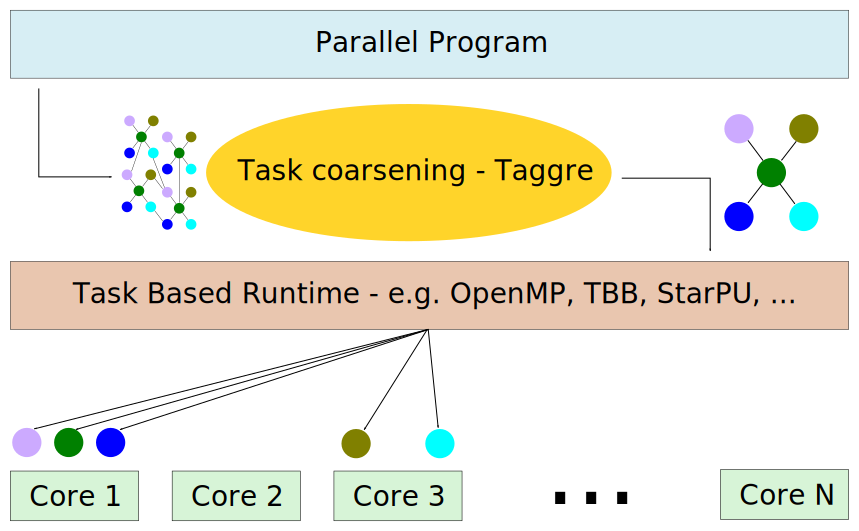
\includegraphics[width=\textwidth]{coarsening}
  \caption{Big pictures of the role of Taggre in a parallel program.}
  \label{fig:taggre}
\end{figure}



%-------------------------------
\section{Aggregate operator algorithms}

As a proof of concept, we have defined several heuristics that
coarse the DAG to change the task grain size.
%% coarsening the grain size of task DAGs.
Multiple heuristics may be
chained together to further coarsen the DAG. In Taggre, each algorithm is
thus designated by a letter. The sequence of selected letters is
called the  {\bf Coarse String}. For example, the Coarse String
``SD(300)F(32)'' means the call of Sequential algorithm, followed
by the Depth Front algorithm with parameter 300 and finally by the
Front algorithm with parameter 32. The parameters are
algorithm-dependent.

\subsection{Sequential (S)}
This is the most straightforward algorithm.
%
We aggregate tasks having a single predecessor with their predecessor, if such a predecessor has a single successor (Fig.~\ref{fig:S_algo}).
%   (-_-)   %
\begin{figure}[!ht]
  \centering
  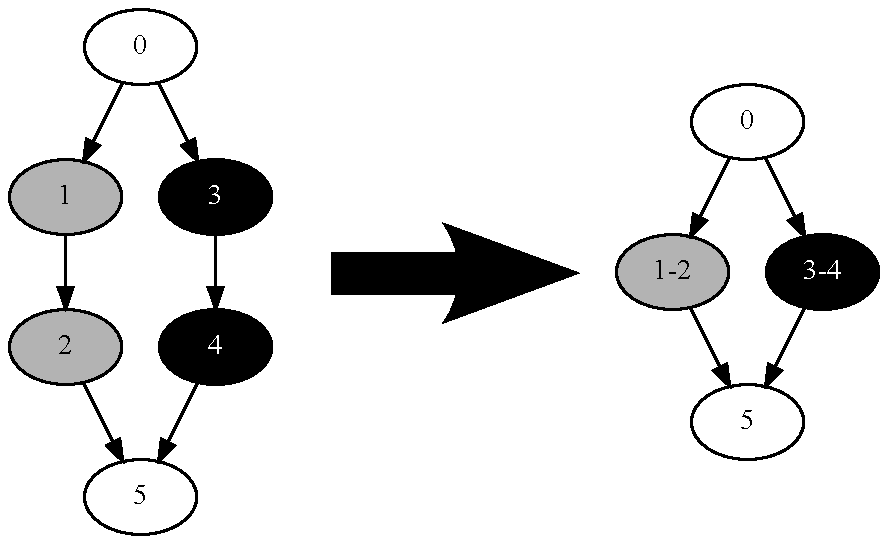
\includegraphics[width=3in]{algo_S}
  \caption{Example of aggregation with S algorithm}
  \label{fig:S_algo}
\end{figure}


\subsection{Front (F)}
This algorithm takes one argument which is the maximum number of
tasks per depth level. We call this number $N$. The basic idea of
this algorithm is to limit the number of simultaneously available
tasks and thus to limit the oversubscription of computing units.
To do this, the Front algorithm implements a breadth-first traversal
of the DAG. During the traversal, it aggregates tasks of same
depth to build up to the maximum of $N$ coarse tasks of similar computation
time (e.g., grain size) per depth (Fig.~\ref{fig:F_algo}).

\begin{figure}[!ht]
  \centering
  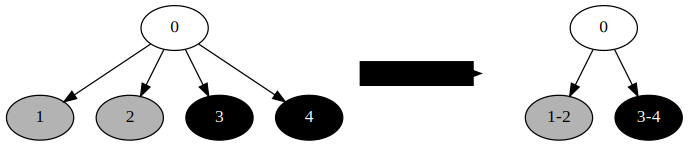
\includegraphics[width=3in]{algo_F2}
  \caption{Example of aggregation with the F algorithm and parameter 2}
  \label{fig:F_algo}
\end{figure}


\subsection{Depth Front (D)}
This algorithm expects one argument which is the maximum number of
fine grain tasks aggregated into a coarse grain task. We call this
number $M$.
The main idea of this algorithm is to aggregate a task with some
of its descendants, up to the limit $M$. For that, the algorithm
performs a breadth-first traversal of the descendants of a task to
aggregate up to $M$ tasks together. However, during the traversal, each new
level encountered is sorted, from the task having the highest
number of predecessors in the current aggregate being built, to
the task having the least predecessors in this aggregate. The
rationale of this heuristics is to favor aggregating tasks that
are more tightly connected in the DAG (Fig.~\ref{fig:D_algo}).


The first loop of Algorithm~\ref{depth_front_algo} is a loop for each
level of the coarsened DAG.

The second loop is a loop over tasks of the same level in coarsened DAG.
Other tasks will be aggregated to these tasks in the third loop, we call them
{\em Master} and they will be kept in the final DAG.

The third loop is the aggregation loop, we aggregate tasks descendants of
the {\em Master} task to it.

\begin{algorithm}
  \caption{Depth Front}
  \label{depth_front_algo}
  \begin{algorithmic}
    \REQUIRE $M$, DAG
    \STATE Ready = empty list
    \STATE put root tasks of DAG in Ready
    \WHILE{Ready not empty}
    \STATE Depth = Ready
    \STATE Ready = empty list
    \WHILE{Depth is not empty}
    \STATE Master = pop first from Depth
%    \STATE DAG\_tmp = DAG.clone()
    \STATE Release = empty list
    \STATE put Master in Release
    \STATE count: 0
    \WHILE{$count < M$ AND Release is not empty}
    \STATE Next = pop first from Release
    \STATE count++
    \STATE aggregate Master and Next
    \STATE put tasks released by Next in Release, sorted by
    \STATE \quad number of precedence of Master
    \ENDWHILE
    \STATE put tasks released by Master in Depth
    \ENDWHILE
    \STATE put tasks released by Depth in Ready
    \ENDWHILE
  \end{algorithmic}
\end{algorithm}

\begin{figure}[!ht]
  \centering
  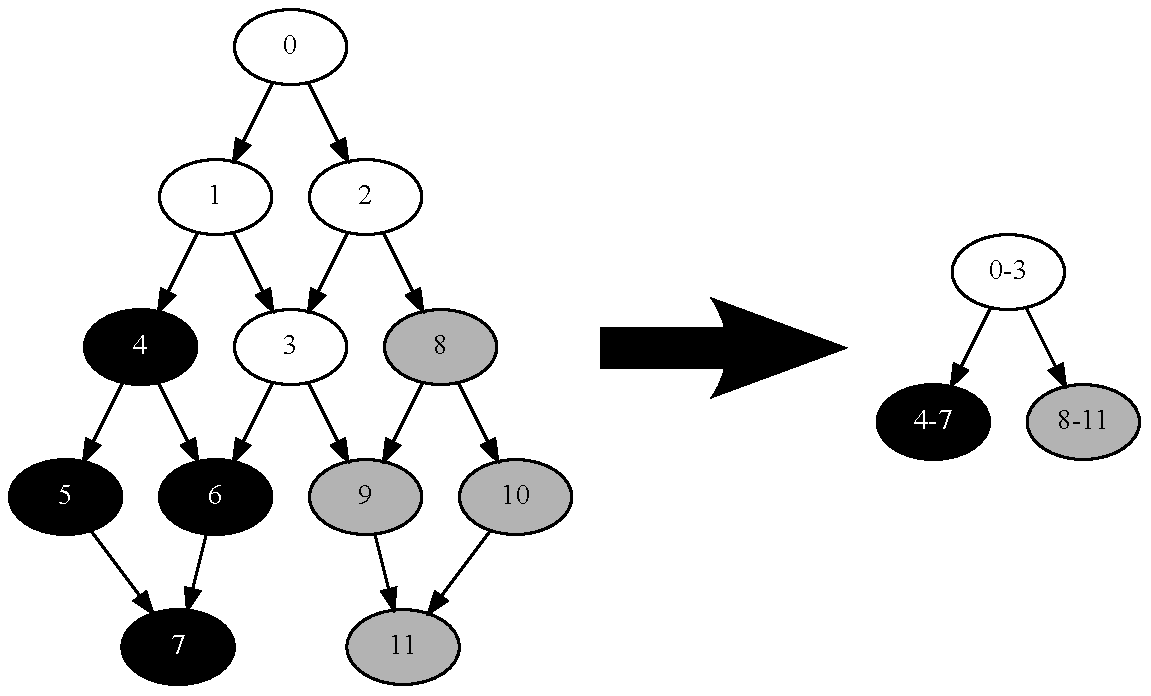
\includegraphics[width=3in]{algo_2}
  \caption{Example of aggregation with D algorithm and parameter 4}
  \label{fig:D_algo}
\end{figure}

\subsection{Continuation Oriented (C)}
The Continuation Oriented algorithm is an aggregation method which improves
serial accesses to data inside an aggregated task. For a 3D cube,
it's equivalent to putting tasks with the same (x,y) coordinates together.

%% To begin, the user must register an identifier on each tasks with the constraint
%% of following identifier have data that follow. Then the Cache Oriented algorithm
%% aggregate tasks with continuous identifier if a dependency exist between them.
%% This algorithm couldn't be use on all DAG, in some of them, this aggregation
%% will form cycle dependencies and the coarsed graph can't be execute.




\section{Example of utilization}
\subsection{High breath graph}
High breath graph have a lot parallelism, so we can group tasks which have the same depth.
The Front algorithm do it well bu the integer parameter is a little hard to find, we need
to keep enough parallelism in order to use all cores but we also want to reduce the number
of tasks.
Empirically I found a value of about three times the number of cores.

\subsection{Tree}
With a tree, we begin with.

\subsection{Diamond}
In a diamond graph, nodes are highly connected but connections are spatially close.


We can found this type of graph in 2D physical simulation.

\subsection{3D simulation}
For the 3D case, the Continuation Oriented algorithm allows to reduce the problem to a Diamond case problem.
